\subsubsection{Gate-Treiber}
\label{subsubsec:Gate-Treiber}

%Nebst dem TMC4671, welcher für die Ansteuerung benötigt wird, braucht es für die Magnetisierung der Spulen des BLDC-Motors eine Schaltlogik. Dabei Handelt es sich um den TMC6200. Dieser ist eine umfangreiche Ergänzung zum TMC4671. Auf den TMC6200 und weitere benötigte Komponenten wird im folgenden eingegangen.
%\subsubsection{Problem}\label{subsubsec:Problem_TMC6200}

Der Motor wird über eine H-Brücke gesteuert. Dies bedingt pro Spule zwei MOSFET's, um diese entsprechend magnetisieren zu können. Um einen MOSFET in einen leitenden Zustand zu bringen, muss das Gate des MOSFET's mit einer elektrischen Ladung gefüllt werden. Während diesem Vorgang hat am Gate ein kapazitives Verhalten, was bedeutet, dass bei jedem Schaltvorgang Ströme fliessen. Um ein optimales Schaltverhalten zu erreichen, die Umschaltverluste zu verringern und somit die daraus entstehende Abwärme zu verhindern, ist es vorteilhaft die Gates so schnell wie möglich laden und entladen zu können. Da kommt der Gate-Treiber ins Spiel. Dieser ladet und entladet das Gate schnell genug und stellt die dazu benötigte Energie für das Gate zur Verfügung.

\paragraph{Schema}\mbox{}\\

Damit ein Aufbau mit mehreren Gate-Treibern vermieden werden kann und einige Zusatzfunktionen wie Strommessung, Messverstärkung, Kurzschlussdetektion etc. genutzt werden können, wurde während des Entwicklungsprozesses ein Gate-Treiber von Trinamic ausgewählt. Das entsprechende Bauteil ist der TMC6200. Das Blockdiagramm und eine Beispielschaltung befinden sich im Anhang Kapitel \ref{Appendix:Schaltung_TMC6200} und \ref{Appendix:Blockdiagramm_TMC6200}. Das Blockdiagramm zeigt, dass der TMC6200 aus einer Treiber-Logik für den Motor, einem SPI-/Pinsettings-Interface, einer Diagnosenlogik, Strommessschaltung und diversen unterstützenden Schaltungen wie Spannungsversogrung besteht. Das Schema ist in Abbildung \ref{fig:Schema_Gate_Treiber} zu sehen.


\begin{figure}[H]
	\centering
	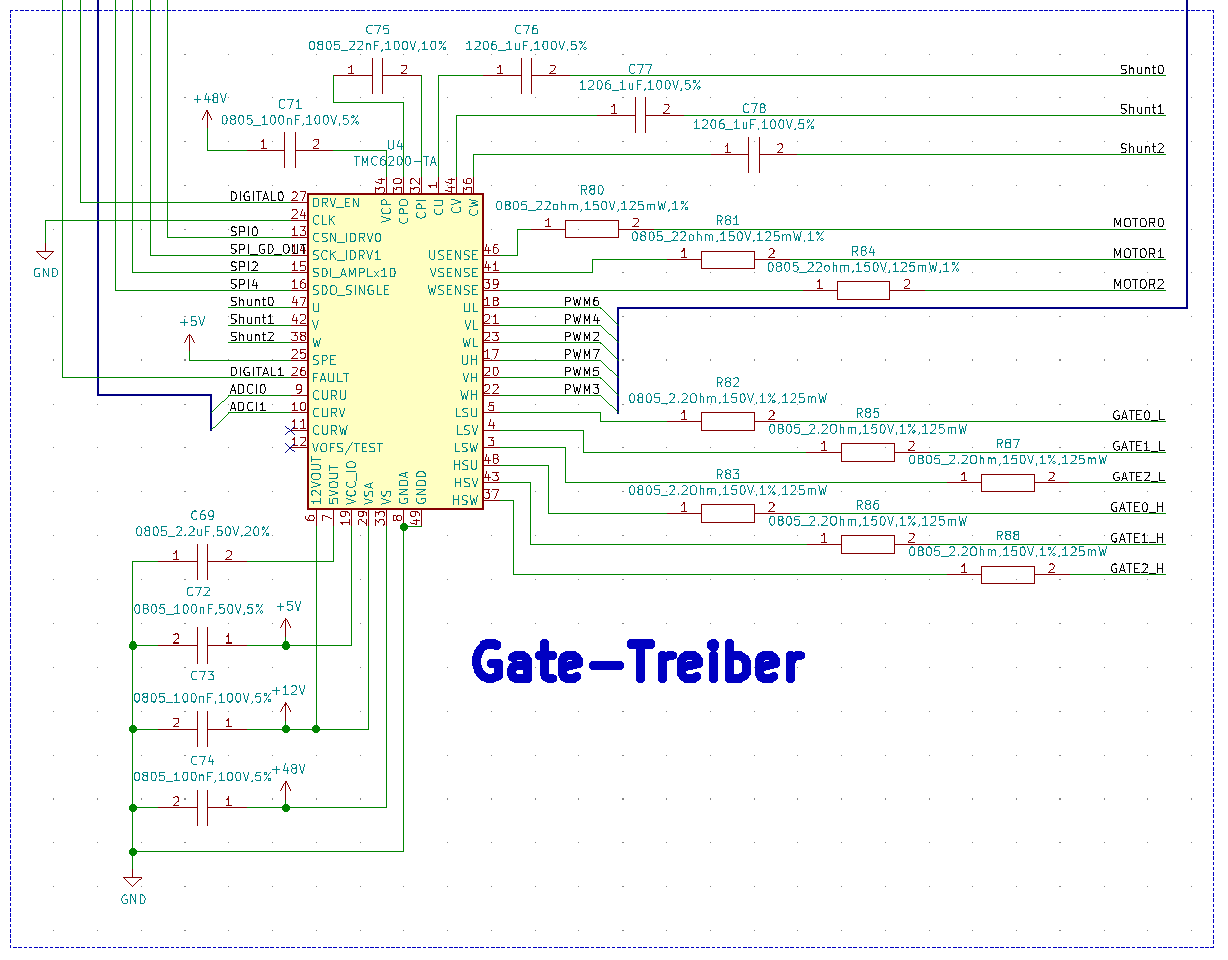
\includegraphics[width=\textwidth]{graphics/Schema_Gate_Treiber}
	\caption{Schema Gate-Treiber.}
	\label{fig:Schema_Gate_Treiber}
\end{figure}

%\begin{figure}[h!]
%	\centering
%	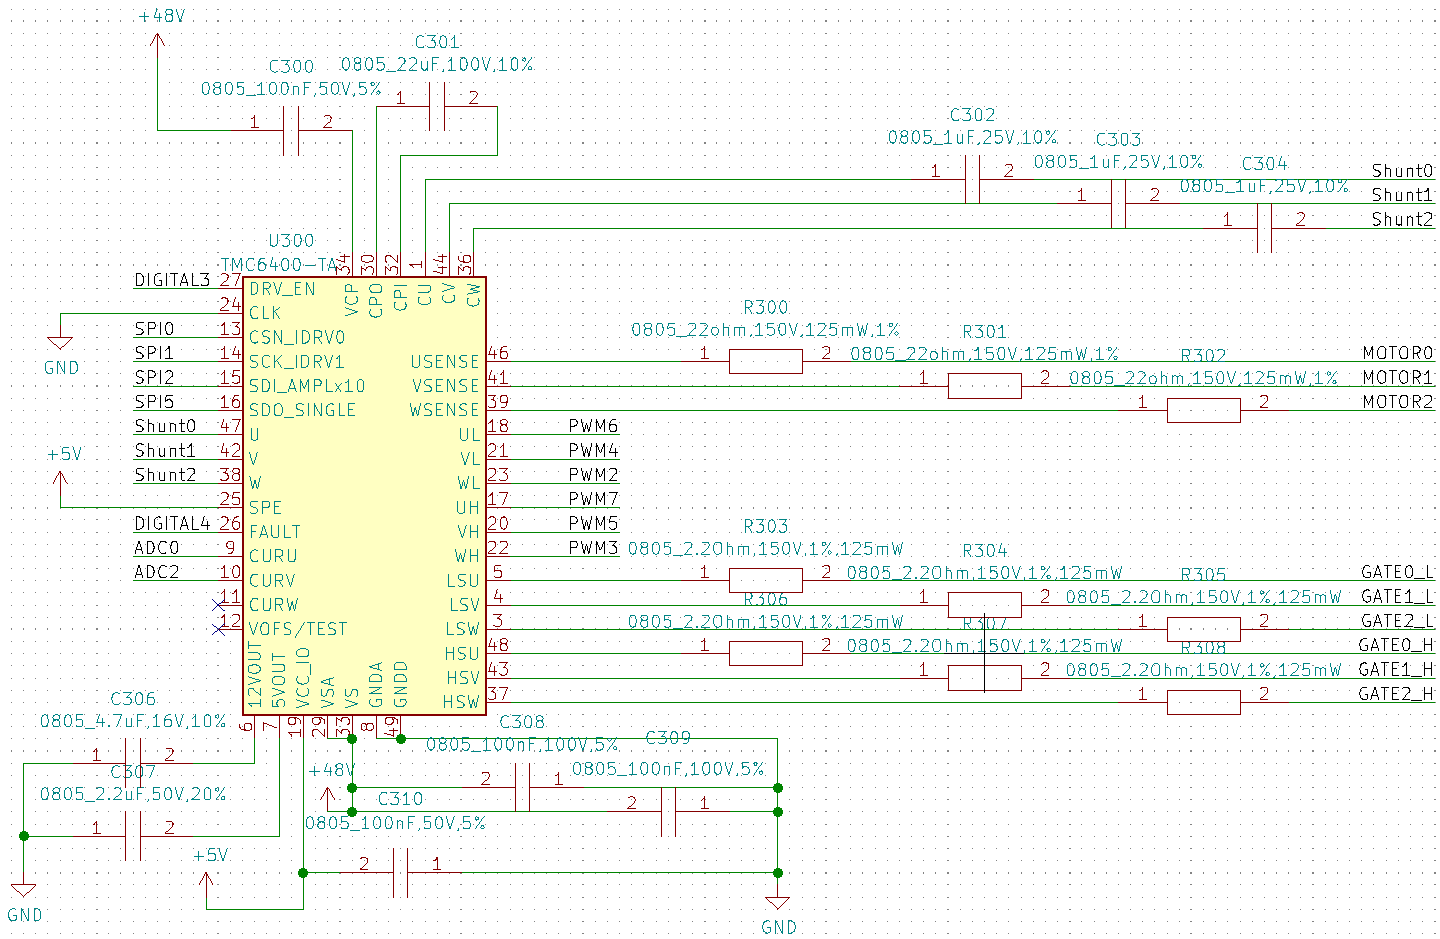
\includegraphics[width=0.8\textwidth]{graphics/TMC6200_Schema.png}
%	\caption{Teilschema Ansteuerung Motor. Hier Gate-Treiber-IC TMC6200.}
%	\label{fig:Schema_TMC6200}
%\end{figure}
%\begin{figure}[h!]
%	\centering
%	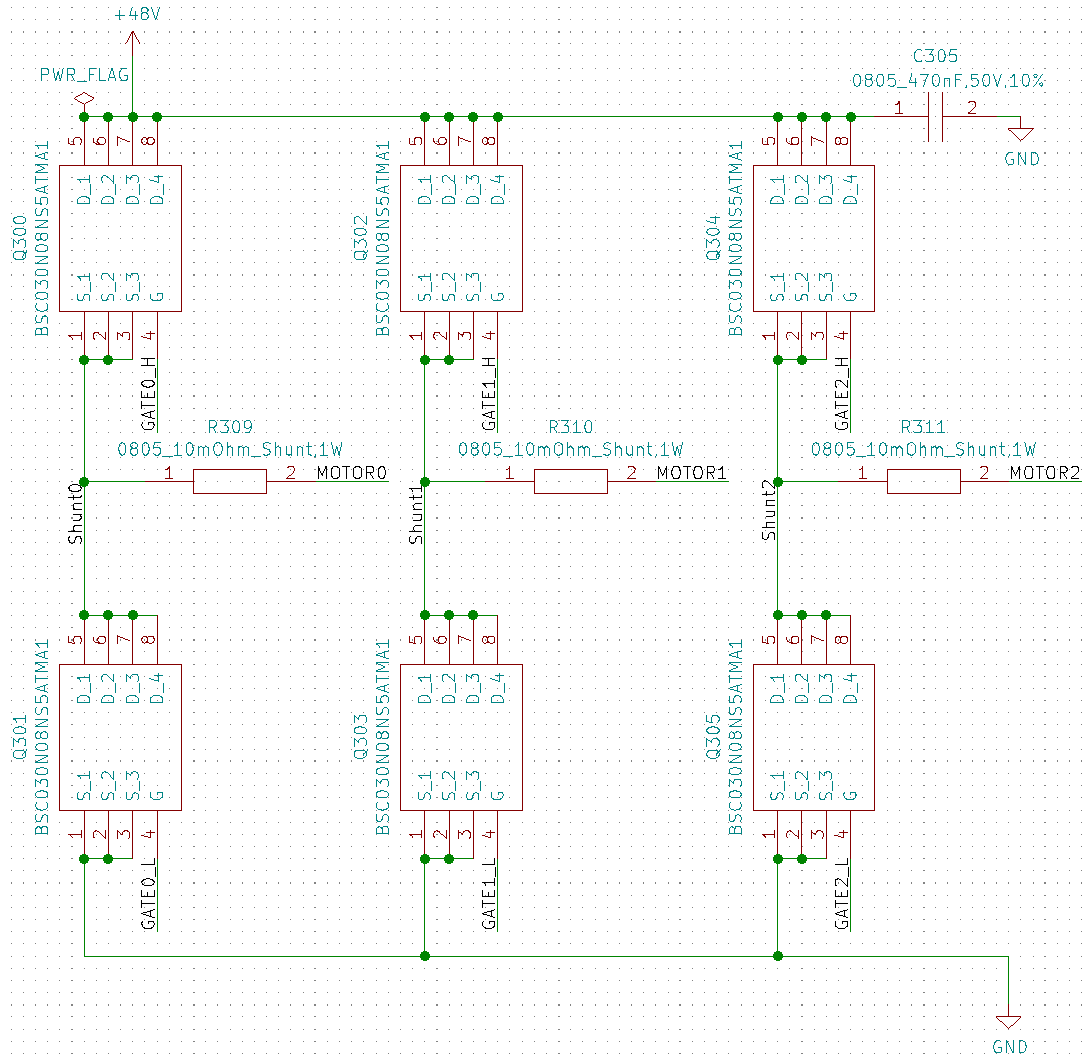
\includegraphics[width=0.6\textwidth]{graphics/H_Bruecke_Schema.png}
%	\caption{Teilschema Ansteuerung Motor. Hier H-Brücke.}
%	\label{fig:Schema_TMC6200}
%\end{figure}

\paragraph{Funktionsbeschrieb der Schaltung}\mbox{}\\

%\subparagraph{Shunt-Widerstände $\mathrm{\mathbf{R_{Sense}}}$}
Für die Messung des Stromes wird ein Shunt in Serie mit der Spule des BLDC-Motors geschaltet. Die Shunts R89 - R91 sind in Abbildung \ref{fig:Schema_H_Bruecke_und_BLDC} zu sehen. Durch den fliessenden Strom liegt eine Spannung über dem Shunt, welche dann vom TMC6200 verstärkt wird und aufbereitet an den Kontroll-Chip TMC4671 ausgegeben wird. Die Verstärkung sowie Offset auf das Signal sind über SPI programmierbar.
Die Dimensionierung der Widerstände und die darauf folgende Programmierung des TMC6200 sind schon von Trinamic ermittelt worden. Es wird empfohlen, die Widerstände nach dem Maximalstrom des Motors auszuwählen. Im Falle des AKM22h sind dies 5A. Darüber hinaus wird empfohlen, eine Überdimensionierung von 25-50\% vorzunehmen. Die Schaltung für den PartyMixer wird auf 10A ausgelegt. Eine von Trinamic erstellte Tabelle  empfiehlt einen Widerstand von 10m\textOmega\ für die Shunt-Widerstände und einen Verstärkungsfaktor der Phasenströme von 10. Die Tabelle ist im Anhang Kapitel \ref{Appendix:Shunt} zu finden. \cite[S.31]{trinamicmotion_control_gmbh__co_kg_tmc6200_2019}

%\begin{tabular}{lll}
%$\mathbf{R_{Sense}}$ =  \textbf{10m\textOmega}\\
%\textbf{Verstärkungsfaktor}= \textbf{10x}   
%\end{tabular}

%\paragraph{Gate Vorwiderstände $\mathrm{\mathbf{R_{Gate}}}$}

Da das Gate ein kapazitives Verhalten zeigt, ist der Strom, welcher zu Beginn ins Gate fliesst, sehr hoch. Der Gate-Vorwiderstand begrenzt diesen, um das Gate und den Pin des TMC6200 vor Überströmen zu schützen. Die Vorwiderstände R82 - R83 und R85 - R88 sind in Abbildung \ref{fig:Schema_Gate_Treiber} zu sehen.
Die Dimensionierung der Gate-Widerständen wurde an die MOSFET Gate-Drain-Ladung (Miller charge) angelehnt. Auch in diesem Falle wurden von Trinamic schon einige Parameter ermittelt und im Anhang \ref{Appendix:Gate_Vorwiderstand} dargestellt. Die Gate-Ladung des ausgewählten MOSFET's beträgt 61nC. Aus der Tabelle kann somit ausgelesen werden, dass der Vorwiderstand R$_{Gate}\leq$2.5\textOmega\ sein sollte und das programmierbare Register DRV\_STRENGTH auf 1 bis 3 gesetzt wird. \cite[S.13]{trinamicmotion_control_gmbh__co_kg_tmc6200_2019}

%\begin{tabular}{lll}
%$\mathrm{\mathbf{R_{Gate}}}$ & \textbf{=} & $\mathrm{\mathbf{R_{Gate}\leq2.5\Omega}}$ \\
%\textbf{DRV\_STRENGTH} & \textbf{=} & \textbf{1 bis 3}
%\end{tabular}

%\paragraph{Schutzwiderstände Messeingang $\mathrm{\mathbf{R_{Protect}}}$}

Wird von einem High-Zustand in einen Low-Zustand gewechselt, kann aufgrund von Induktivitäten der Shunts oder deren Verbindungen die Spannung unterschiessen. Der Schutzwiderstand schützt den Messeingang des TMC6200 vor diesem Effekt. Die Schutzwiderstände R80, R81 und R84 sind in Abbildung \ref{fig:Schema_Gate_Treiber} zu finden.
Die Dimensionierung dieses Widerstands wird im Datenblatt mit einem Widerstandswert zwischen 10\textOmega\ und 22\textOmega\ angegeben.\cite[S.10]{trinamicmotion_control_gmbh__co_kg_tmc6200_2019}

%\begin{tabular}{lll}
%$\mathrm{\mathbf{R_{P}}}$ & \textbf{=} & \textbf{10\textOmega\ bis 22\textOmega}\\
%\end{tabular}

%\paragraph{Bootstrap Kondensatoren $\mathrm{\mathbf{C_{Bootstrap}}}$}

Die Bootstrap-Kondensatoren werden benutzt, um die Gate-Spannung am High-Side-MOSFET auf die Schaltspannung (48V) plus die Gatespannung anzuheben. Die Kondensatoren C76 - C78 in Abb. \ref{fig:Schema_Gate_Treiber} unterstützen diesen Effekt.
Die Dimensionierung dieser Kondensatoren wird im Datenblatt mit einem Kapazitätswert zwischen 470nF und 1\textmugreek F angegeben, bei einer Nennspannung von 16V oder 25V. Weiter gilt gemäss Datenblatt, dass bei MOSFET's mit einem $\mathrm{Q_G \geq 40nC}$ die Gatekapazität 1\textmugreek F sein soll. Da die Kapazität 61nF beträgt, ist dies der Fall. Die Bootstrap-Kondensatoren werden deswegen mit 1\textmugreek F dimensioniert. \cite[S.10]{trinamicmotion_control_gmbh__co_kg_tmc6200_2019}

%\begin{tabular}{lll}
%$\mathrm{\mathbf{C_{Bootstrap}}}$ & \textbf{=} & \textbf{1\textmugreek F (25V)}\\
%\end{tabular}

%\paragraph{Externer Gate-Spannungsregler}

Aufgrund der hohen Versorgungsspannug (48V), treten im IC über den Gate- und 5V- Spannungsreglern erhebliche Verluste auf. Um diese Verluste zu reduzieren, wird gemäss Datenblatt \cite[S.11]{trinamicmotion_control_gmbh__co_kg_tmc6200_2019} geraten, eine externe Gate-Spannung anzuhängen. Für beste Resultate wird eine Spannung von 12V $\pm$ 1V empfohlen.
Die Dimensionierung der benötigten Kondensatoren ist im Anhang Kapitel \ref{Appendix:Gate_Spannungsversorgung} zu finden. Für den Kondensator C69 sollten 2.2\textmugreek F verwendet werden und für den Kondensator C73 100nF.

%\begin{tabular}{lll}
%$\mathrm{\mathbf{C_{69}}}$ & \textbf{=} & \textbf{2.2\textmugreek F}\\
%$\mathrm{\mathbf{C_{73}}}$ & \textbf{=} & \textbf{100nF}\\
%\end{tabular}